\section{MPI One-Sided Communication}
\subsection{Required submission files}
\begin{enumerate}
  \item \hl{The updated \emph{gauss.c} file.}
  
  \verb!Data/io/gauss.c! and \verb!Data/io/mgen.c!
  
  There is an updated \verb!mgen.c! matrix generator which generates binary matrices.
  \emph{Please use this to generate matrices to run the code as it only accepts binary input!}

  \item \hl{The new performance plots and description in the report.}
  
  The figures are in Fig. \ref{fig:par_io_io_vs_domain}, \ref{fig:par_io_io_vs_proc},
  \ref{fig:par_io_total_vs_domain}, \ref{fig:par_io_total_vs_proc}, \ref{fig:par_io_vampir}.

\end{enumerate}

\subsection{Questions}
\begin{enumerate}
  \item \hl{Which MPI-IO operations were applied to transform the code? Explain your choices.}
  There were several MPI-IO operations chosen to replace different parts of the code
  \begin{enumerate}
  \item Reading in the matrix.
  
  We decided to read and write the matrix data in binary format instead of ASCII, because it decrease amount of data to be read
  and also ease creating offsets for different proccesses. We used one byte integer to write matrix and vector entries
  since in original mgen.c file range of their values is from 0 to 100.


  We used an \verb!MPI_Read! function to read the first two ints at the beginning of the matrix to determine matrix dimensions.
  This allows us to eliminate blocking broadcast in the beginning of the io phase.

  We then used an \verb!MPI_File_set_view! to separate the file into chunks and an \verb!MPI_File_read_all! for all 
  processes to read in the required matrix data. We decided to use this functions because MPI documentation claims
  that this function allows to get the biggest io bandwith compared to all other functions.
  
  We used \verb!MPI_File_set_view! and \verb!MPI_Read_all! to read in the rhs data as well.
  
  \item Writing the resulting solution vector
  We used an \verb!MPI_Write! in the root process to store the output vector size. We then used \verb!MPI_File_set_view!
  and \verb!MPI_Write_all! so that each process could write to the correct segment in the file. Since resulting vector 
  is a floating point array we wrote the resulting vector using binary representation of double.
  
  \end{enumerate}
  
  \item \hl{What is "Data Sieving" and "2-Phase IO"? How do they help improve IO
performance?}
	\begin{enumerate}
	\item Data Sieving
	
	Data sieving is performed when multiple non-contiguous chunks of data are 
	requested by a single process. Instead of multiple small accesses, these accesses are aggregated and  a large contiguous chunk of data (containing all necessary data) is read into a memory buffer. The required chunks of non-contiguous data can then be read from or written to in the buffer. The entire buffer can then be written back to the filesystem if write operations have taken place. Note that the
	large contiguous chunk of data must be locked to prevent memory inconsistencies during write operations.
	
	The possible benefits are that, individual memory accesses for a large number of small, non-contiguous data chunks takes a significant amount of time. It is far better to make a single large call to memory as this will reduce the overhead from repeated communications. However, the downside is the large amount memory required as a larger chunk is loaded into memory than needed.
	
	\item 2-Phase IO
	
	This is also known as collective buffering and is performed during non-contiguous memory access
	by multiple processes. File accesses are performed by specific processes where data is 
  aggregated. This works for both reading and writing. When reading, only certain processes will read large chunks of 
  contiguous data---which is then communicated to the necessary processes. When writing, large chunks of data are 
  aggregated in specific processes, which then write to file.
	
	Effectively, this ensures that file accesses are large and contiguous, significantly reducing IO time as opposed to performing many file accesses to small chunks of non-contiguous data. This does incur an additional communication cost/step but IO access is often far slower and the benefits of large contiguous file access outweights that of communication.
	\end{enumerate}

  \item \hl{Was the original implementation scalable in terms of IO performance?}
  The original implementation was not scalable in terms of IO performance. Only one process would read or write data. 
  Thus, time would remain the same for IO regardless of the number of MPI processes.
  
  \item \hl{Was the original implementation scalable in terms of RAM storage?}
  The original implementation was not scalable in terms of RAM. 
  When the program is run on a distributed memory system the entire matrix must fit inside the RAM associated with 
  the processing unit executing the root process. This problem would not change regardless of the number of 
  processing units (with their own memory) added.
  
  \item \hl{How much of the communication in the application was replaced or eliminated with MPI-IO? (Use
Vampir)}

  Using a parallel io allowed elimination of all of the communication during initialization phase completely.

  Initial send of the matrix sizes was replaced with all of the processes reading it from the file.

  Broadcasting of the matrix for each individual process is no longer needed since all of the processes read their own 
  part from file. Same holds for vector rhs.

  The results of execution of the parallel io code can be seen in the figure \ref{fig:par_io_vampir}. It can be seen
  that there is no sending or recieving data using explicit send or recieve functions present.

  \item \hl{Were there any performance improvements due to the change to MPI-IO?}
  
  Yes, there was drastic performance improvements due to MPI-IO. The io time for most of the cases improved over 1000
  times, compared to the baseline as is shown in the figure \ref{fig:par_io_io_vs_proc} and 
  \ref{fig:par_io_io_vs_domain}.

  Since io takes significant amount of time for the baseline implementation of algorithm, it can be seen that 
  total time for all of the runs was up to 5 times shorter for the problem with biggest domain size (figure 
  \ref{fig:par_io_total_vs_proc} and \ref{fig:par_io_total_vs_domain}).

  Using vampir, we can examine that total loading time for the biggest size problem was 0.2 seconds comparing to 15 seconds
  for the baseline (figure \ref{fig:par_io_vampir} and \ref{fig:vampir_baseline}).

  \begin{figure}[p] % h=here, t=top, b=bottom, p=(extra)page, !=force
    \begin{center}
      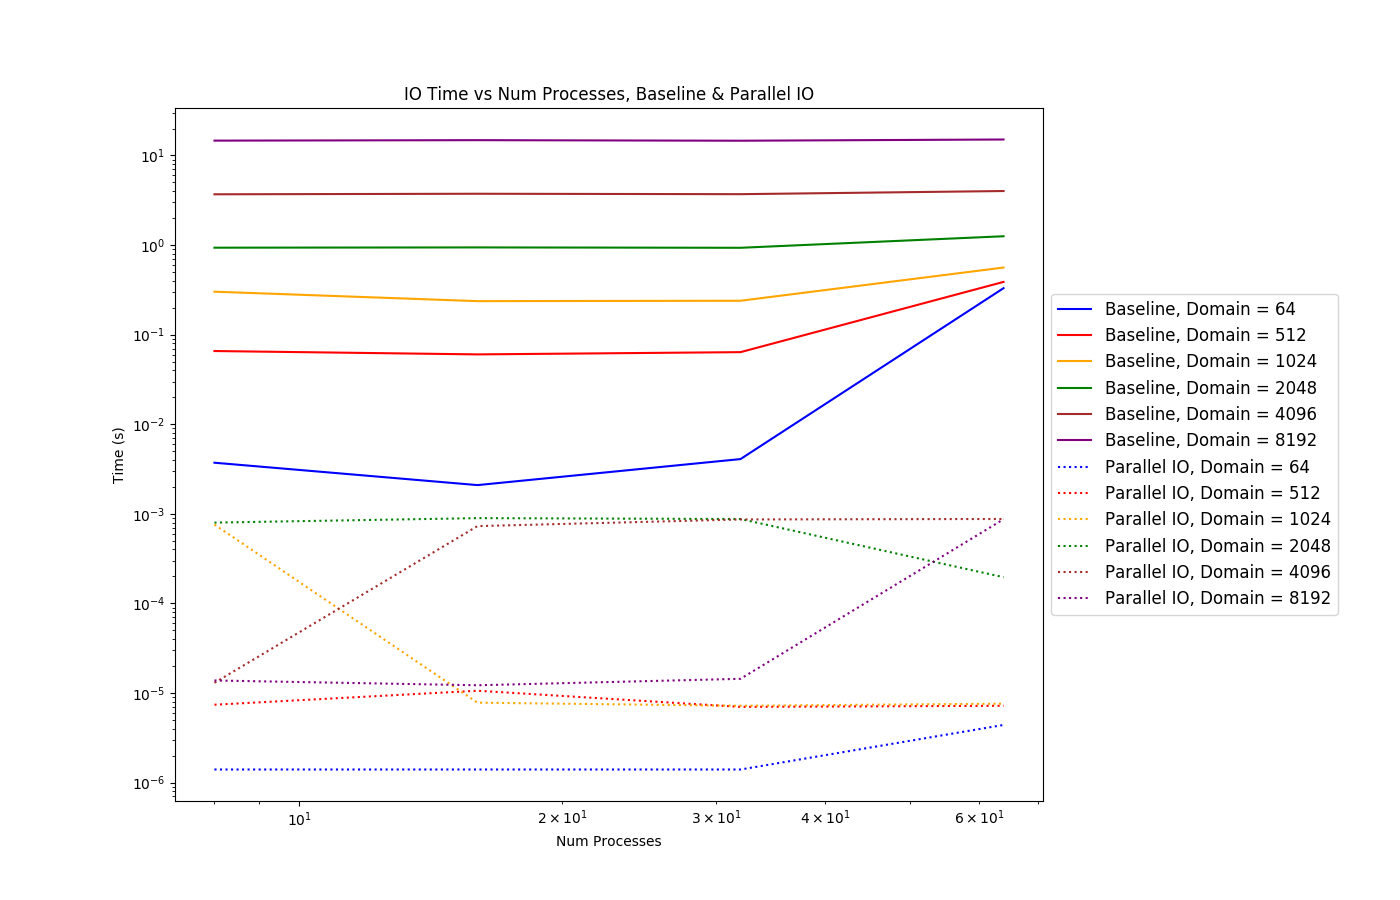
\includegraphics[width=.9\linewidth]{Figures/io/io_multdomain_haswell_io_baseline.png} % It searches in the Figures/ folder!
      \caption{IO time vs \#Processors for baseline and parallel IO}
      \label{fig:par_io_io_vs_proc}
    \end{center}
 \end{figure}
 
 
 \begin{figure}[p] % h=here, t=top, b=bottom, p=(extra)page, !=force
  \begin{center}
    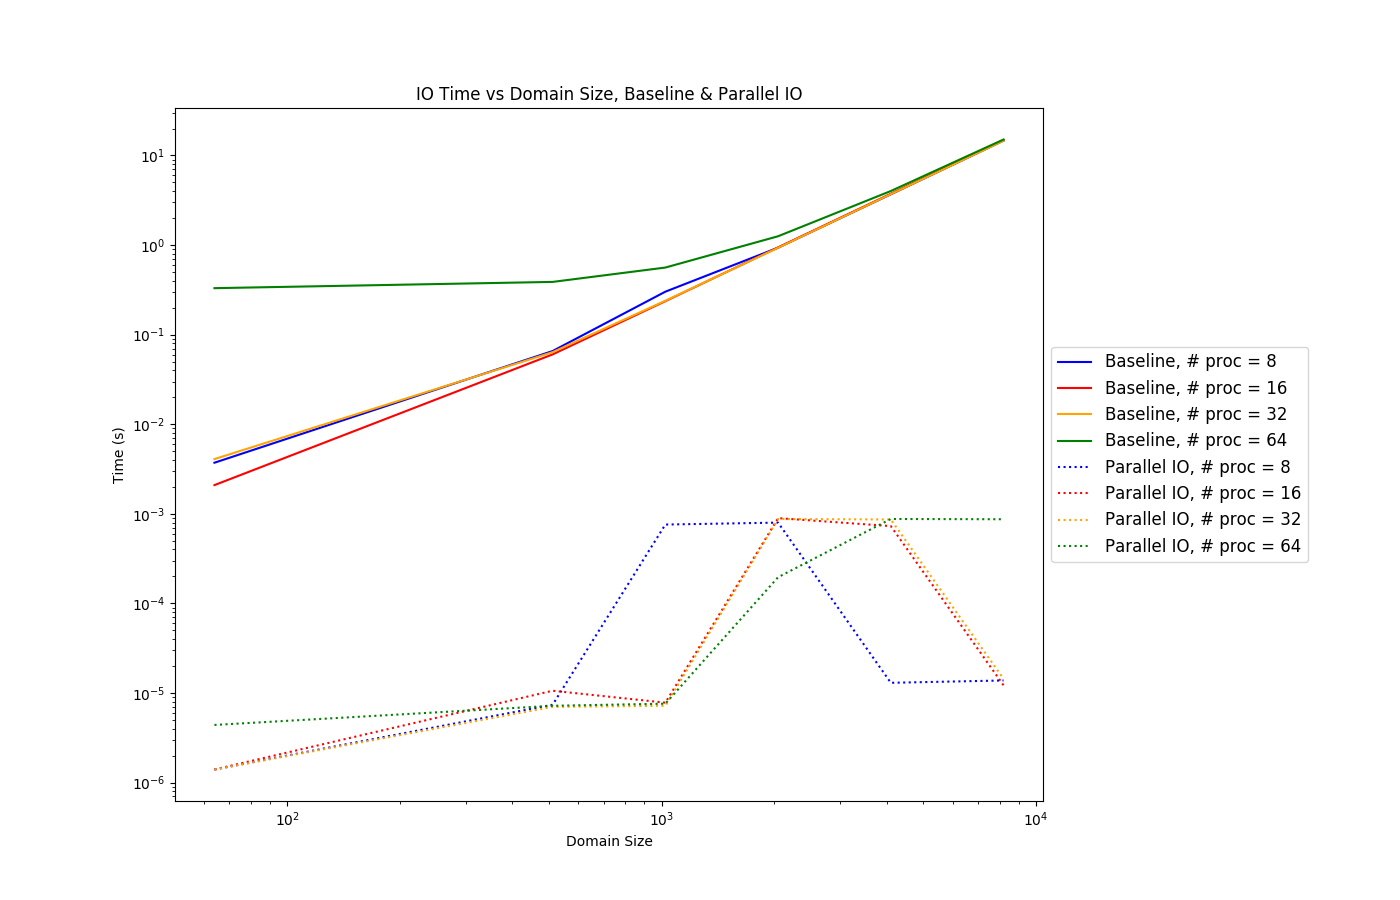
\includegraphics[width=.9\linewidth]{Figures/io/io_multproc_haswell_io_baseline.png} % It searches in the Figures/ folder!
    \caption{IO time vs Domain size for baseline and parallel IO}
    \label{fig:par_io_io_vs_domain}
  \end{center}
\end{figure}
 

 \begin{figure}[p] % h=here, t=top, b=bottom, p=(extra)page, !=force
   \begin{center}
     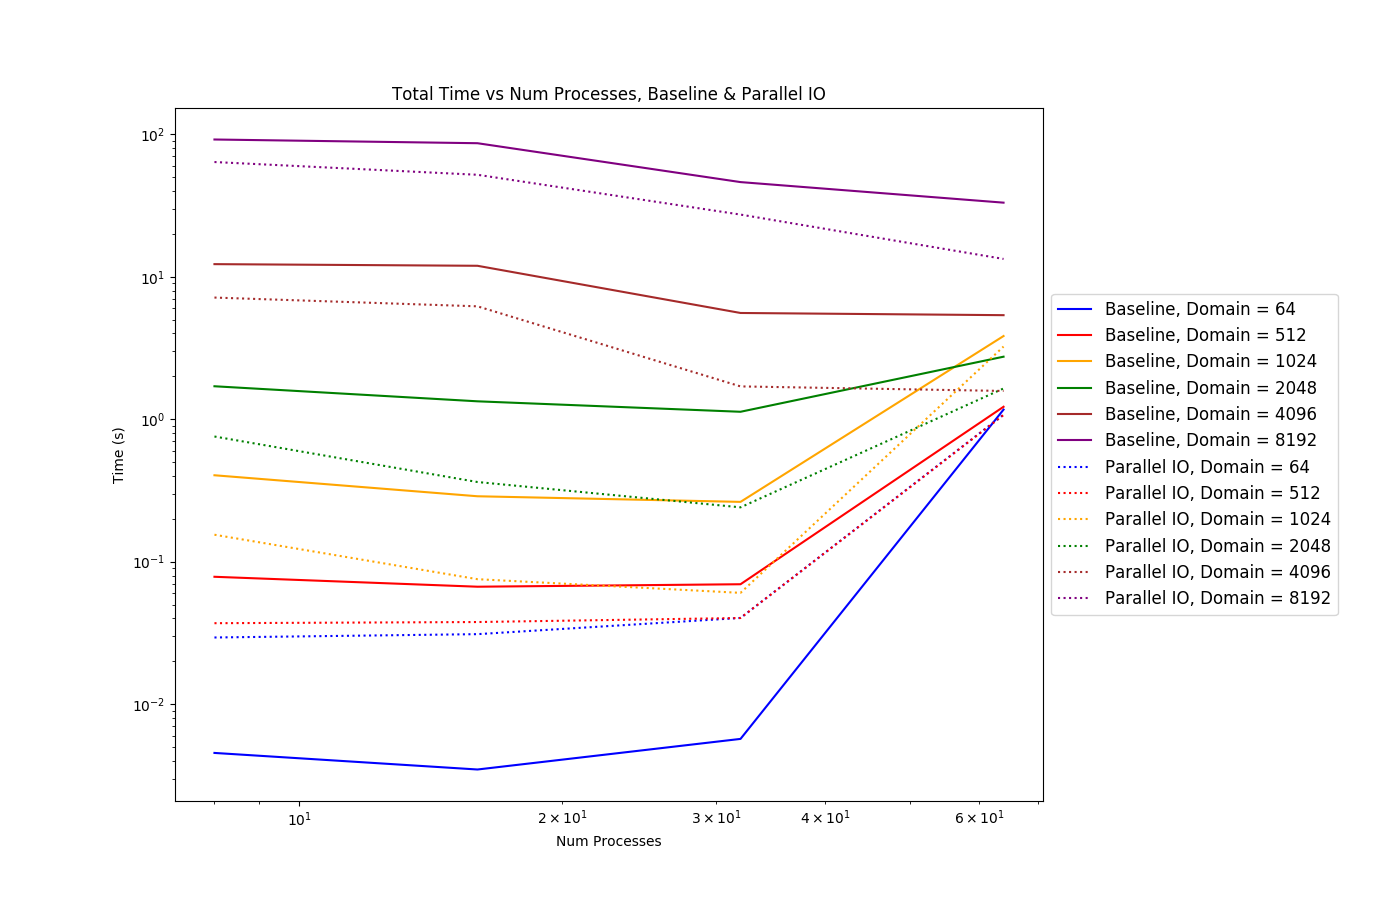
\includegraphics[width=.9\linewidth]{Figures/io/total_multdomain_haswell_io_baseline.png} % It searches in the Figures/ folder!
     \caption{Total time vs \#Processors for baseline and parallel IO}
     \label{fig:par_io_total_vs_proc}
   \end{center}
 \end{figure}

 \begin{figure}[p] % h=here, t=top, b=bottom, p=(extra)page, !=force
  \begin{center}
    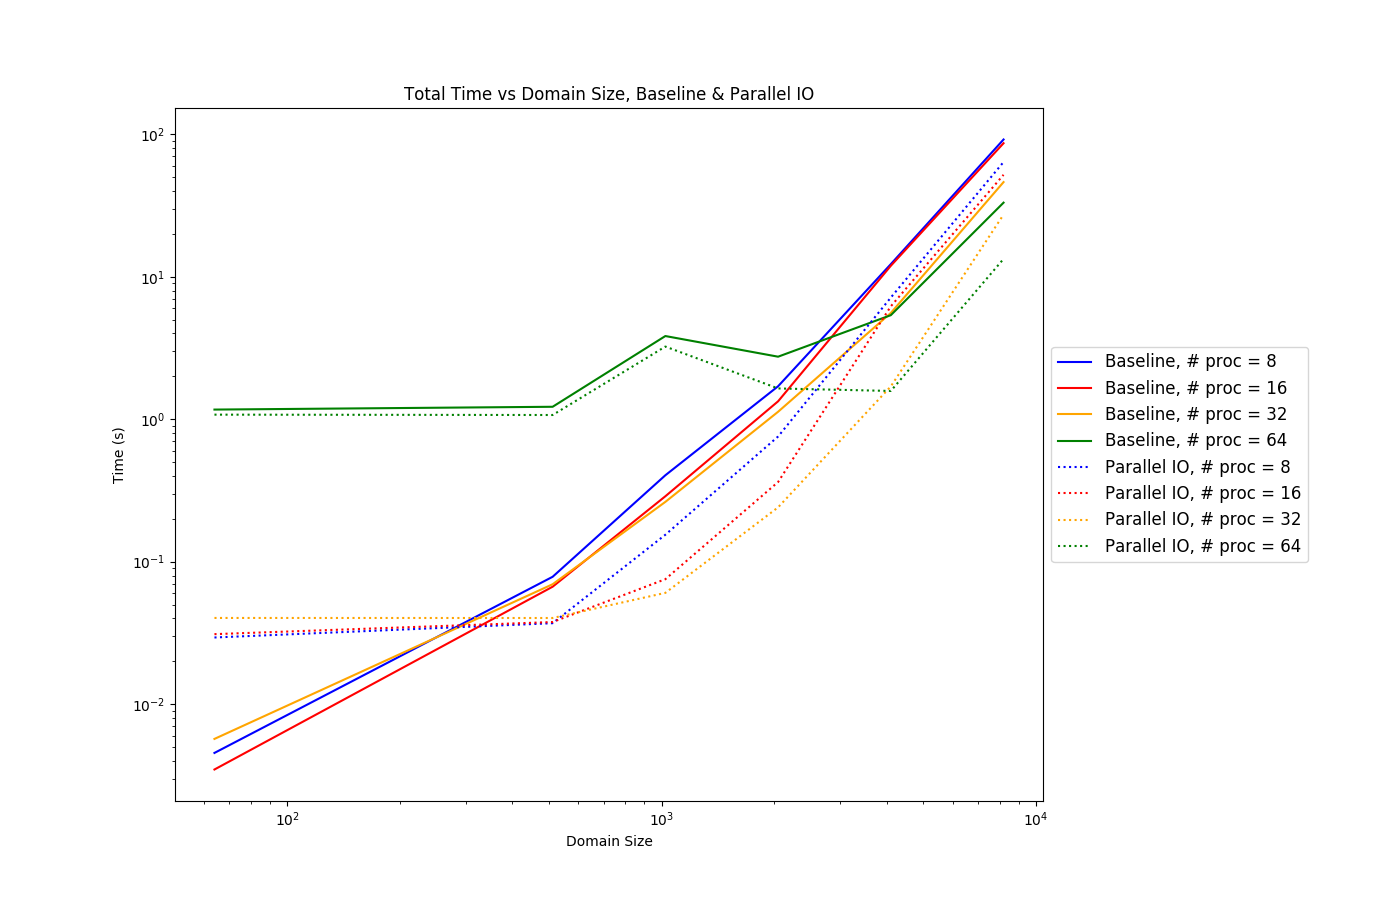
\includegraphics[width=.9\linewidth]{Figures/io/total_multproc_haswell_io_baseline.png} % It searches in the Figures/ folder!
    \caption{Total time vs Domain size for baseline and parallel IO}
    \label{fig:par_io_total_vs_domain}
  \end{center}
  \end{figure}
 
 \begin{figure}[p] % h=here, t=top, b=bottom, p=(extra)page, !=force
   \begin{center}
     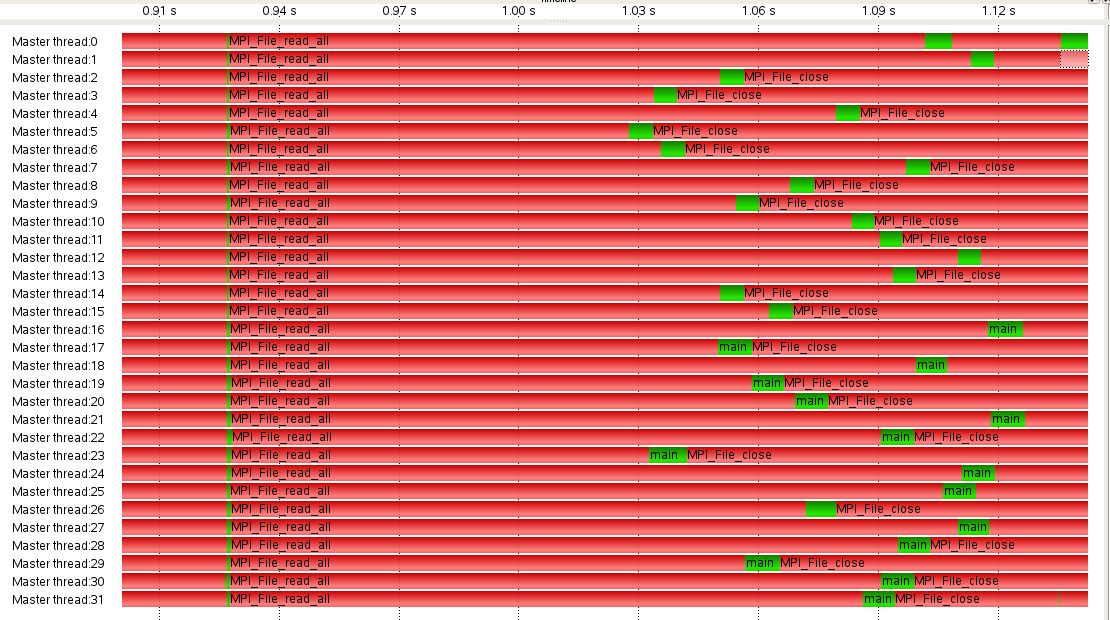
\includegraphics[width=.9\linewidth]{Figures/io/io_vampir_biggest_size.png} % It searches in the Figures/ folder!
     \caption{IO operations in Vampir for the problem size 8192x8192}
     \label{fig:par_io_vampir}
   \end{center}
 \end{figure} 
 
\end{enumerate}

